\documentclass[10pt,conference,compsocconf]{IEEEtran}

\usepackage{hyperref}
\usepackage{graphicx}	% For figure environment


\begin{document}
\title{Higgs Boson Project}

\author{
  Costanza \textbf{Volpini}, Pedro \textbf{Abranches}, Youssef \textbf{Kitane}\\
  \textit{Department of Computer Science, EPFL, Switzerland}
}

\maketitle

\begin{abstract}
    The Higgs boson has many different manners it can decay, we present a robust machine learning model that is able to distinguish between background noise and the possible signal from Higgs boson. Mainly, through data pre-processing and parameter tuning we are able to find which features and parameters best fit our model. A detailed explanation of feature engineering techniques, dataset manipulation and outlier detection is also included in our approach.
\end{abstract}

\section{Introduction}
    From the official ATLAS simulated data we want to be able to find true signals referring to the Higgs boson. To do this, binary classification methods are proved to be better than usual "cut" approaches. Having this in mind, we used several models to make a binary classification based on the given and added features. \\
    After initially testing all the requested machine learning baseline, we focused on improving 2 of them, ridge regression and logistic regression. The latter because it is the one most appropriate for binary classification approaches. And the former because it was a good model to automate its search for best parameters, due to the fast computation that is possible and the low over and under-fitting that it demonstrated when tested with our cross validation function. \\
    The structure of the tests used and all the models and methods used are described in the section \ref{sec:models}. 

\section{Models and Methods}
\subsection{Analysis of the data} \label{sec:models}
From a preliminary visual analysis of the distributions and box-plots of the data regarding the 30 features, we have understood that there exist symmetrical features, some of them having the same values throughout the rows and also a noticeable disparity between features values. Also, through the documentation we have seen how some features are needed for the computation of others and we have taken this into account when designing our approach. \\
A plot of the distributions is shown in Fig. \ref{fig:denoise-fourier}.

\begin{figure}[tbp]
  \centering
  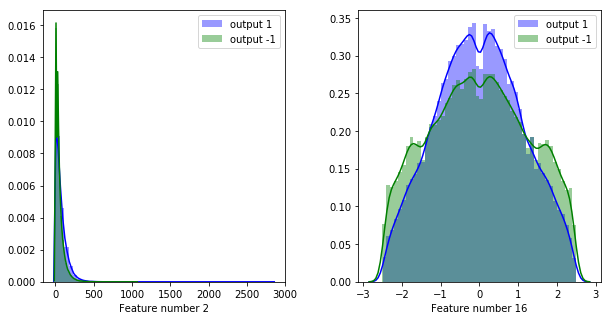
\includegraphics[width=\columnwidth]{dist_plot.png}
  \caption{Distribution of 2 features from the data regarding the classification (noise or background.)}
  \vspace{-3mm}
  \label{fig:denoise-fourier}
\end{figure}


\subsection{Pre-processing of data} \label{sec:models}
A training set (consisting of id columns, 30 feature columns, signal and background labels) and a test set (consisting of id columns and 30 feature columns) are provided.  
Variables that are meaningless or cannot be computed are represented by the value $−999.0$ (out of bounds value), we will denote them \textit{missing values}. \\
We have used the following approaches to pre process the data:
\begin{enumerate}
    \item  \textit{Missing values}: Replace all the missing value by the \textit{mean} and the \textit{median} calculated vertically downwards across rows. Mean and median are computed without taking in account missing values. We also tested replacing all the missing value by zero after normalizing all the variables.
    \item \textit{Outliers detection}: After a brief exploration of the data, we have noticed that some features contain values that could be outliers. We have tested different percentiles, however most of them cut precious feature values. 
    \item \textit{Feature Engineering}: We have used feature correlations to obtain new engineered features, as there could be valuable hidden information based on interaction between the already known features. Other, more realistic, features were created by trying to make sense of the data using the documentation it was provided. An example of these latter features is the transverse momentum ratio of tau-lep to the total transverse momentum. The final approached that we have decided to use for our final submission was to compute the exponential and logarithm of all the features and also splitting each feature by using the median in order to have more parameters to train the algorithm.
    \item \textit{Splitting the dataset}: We have splitted the set taking into account the \textit{PRI\_jet\_num} feature. This feature is responsible of missing variables in other features. We have noticed in fact that if this feature is zero or one then others would be composed just by missing values. We have then divided the set in 4 subset looking on values $0, 1, 2$ and $3$ of the feature. Although we did not use this approach for our final submission, we did several tests having it into account. 
    % % commented out this stuff as we now drop more columns.
    % \iffalse
    % \fi
    \item \textit{Removing columns}: Since there were features containing only constant values, which cannot affect the predictions, at the beginning we have decided to drop them. 
    Referring to the above splitting dataset, we have detected the following features to be dropped (we did not use this approach for our final submission):
        \begin{itemize}
        \item For jet\_num equals to $0$, features: [4, 5, 6, 12, 22, 23, 24, 25, 26, 27, 28, 29]
        \item For jet\_num equals to $1$, features: [4, 5, 6, 12, 22, 26, 27, 28]
        \item For jet\_num equals to $2$ and $3$, feature: [22]
    \end{itemize}
    % We did this also for the new engineered features. 
    \item \textit{Standardization}: After all the transformation on the dataset, the last step was to standardize it. This usually helps to build more robust models, so that extremely big or small values that were not excluded during the outlier removal in some features do not disrupt the weights in a great manner.
\end{enumerate}

\subsection{Methods}
Once the data is pre-processed to have more optimized algorithms, we tried to implement different methods with as a main goal minimizing the given loss function \( \mathcal{L}( w ) \) .
Then we have trained our data-set by applying several methods before testing them.
\begin{enumerate}
\item  \textit{Gradient Descent}: The objective of this algorithm is to minimize the loss function \( \mathcal{L}( w ) \) by updating our weight vector \( \textbf{w} \) using the following formula: 
\begin{equation}
    w^{t+1} = w^{t} - \gamma*\nabla(\mathcal{L}( w^{t} )) 
\end{equation}
The step-size gamma is then normalized:
\begin{equation} \gamma = \frac{\gamma}{\left\| \nabla(\mathcal{L}( w^{t} ))  \right\|} \end{equation}
in order to have a proportional descent slope to the gradient vector.
\item \textit{Stochastic Gradient Descent}: This method is similar to the Gradient Descent but the loss function is calculated on the basis of a sample of the data that we call batch.
In fact, this method allows you to reduce the computational cost but needs more iterations to converge.
\item \textit{Least squares and Ridge regression}:
We implemented the least squares solution \(  w^{*} = (X^{T}X)^{-1}  X^{T} y \)  that satisfies the normal equation \begin{equation}
 X^{T} \underbrace{( y - Xw )}_{\text{error}} = 0
\end{equation}
in order to  minimize the mean squared error \(  \mathcal{L}(w) = \frac{1}{2N}(y - Xw)^{T}(y-Xw) \).
The main problem that comes up with this method is overfitting for relative high degree of augmented features.
In this sense, to deal with a high variance generated by this method, it appears that ridge regression could avoid overfitting by penalizing the loss function with an additional term 
 \( \lambda \left\| w \right\|^{2} \)

 with \( \lambda \) as an hyperparameter.
 \item \textit{Logisitic Regression}:
The main goal of this probabilistic method is to classify our labels into two categories \{-1, 1\}.
Then, we use a sigmoid function \begin{equation} \frac{1}{1+e^{-t}} \end{equation} on which we can apply \( w^{T}.x \) that gives results between 0 and 1.
We predict the posterior probability of \textbf{\textit{y}} given \textbf{\textit{X}} and \textbf{\textit{w}} 
\begin{equation}
    \mathbb{p}(y|X,w) = \prod_{n=1}^{N} \sigma(x^{T}_{n}w)^{y_{n}}[1 - \sigma(x^{T}_{n}w)]^{1 - y_{n}}
\end{equation}
to belong to one or another class and present the loss function as the negative logarithm of this total probability.
In order to update the weight vector \textbf{\textit{w}},  we use both gradient descent and stochastic gradient descent algorithms.
To improve the convergence ratio, we use an other hyperparameter \( \lambda \)  which is  penalizing values of our weight vector \textbf{\textit{w}} that are abnormally high. 
 \end{enumerate}
\section{Results}
By using cross validation the best model that we got is the \textit{ridge regession} with an accuracy of $\approx 0.80$, a model that needed few changes in the original dataset to have a good performance. At the beginning we did a feature augmentation in order to have more parameters to train the algorithm and approximate more complex function.

\section{Discussion}
Using the six methods provided, to obtain good results, one must make a good preprocessing of the data and try to figure out the best hyper parameters. There is room for improvement when it comes to the parameterization as we tested small intervals, and perhaps, for logistic regression, we were stabilizing the loss function in a local minimum. Being this the reason why our last submission is based in ridge regression, a simple method that could get more than 80\% of the correct answers.

\section{Summary}
The project taught us that sometimes a simple well constructed model is better than more complex ones where the data can affect its accuracy. We now have a better understanding of how important the preprocessing is in order to feed data to the model so we can achieve good predictions. Most importantly, we have seen the good use of machine learning to an important problem in another field.

\end{document}
